\subsection{Riparazione per irraggiamento}
\begin{frame}\frametitle{Riparazione per irraggiamento}
\begin{columns}
 \column{0.65\linewidth}
Il sistema in figura è \textbf{eterogeneo}. 

Probabilmente alla rottura o all'irraggiamento viene \textbf{rotto l'ossetano ed il ponte cerchiato in figura}; si ha poi una \textbf{nuova reticolazione} favorita dall'irraggiamento UV.

La riparazione \textbf{non può ripetersi} nello stesso punto.


 \column{0.35\linewidth}
\begin{figure}{\centering{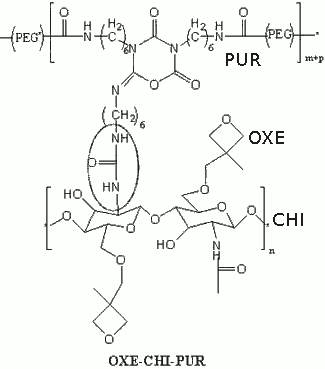
\includegraphics[width=1\textwidth]{altro/oxe-chi-pur.png}}}\end{figure}
\end{columns}
\footnote{\tiny  \fullcite{ottico}}

\end{frame}





\subsection{Riparazione per riscaldamento resistivo}
\begin{frame}\frametitle{Riparazione per riscaldamento resistivo}
\textbf{Scaldando} un filo di materiale \textbf{tramite passaggio di corrente} si ha un \textbf{riscaldamento maggiore} nelle zone in cui sono presenti delle fratture.

Il \textbf{polimero organometallico} riportato in figura è conduttore e può polimerizzare e depolimerizzare facilmente.

Alternative più semplici considerano materiali più comuni rinforzati da \textbf{fibra di carbonio che funge da conduttore}.
\begin{columns}
 \column{0.6\linewidth}
\begin{figure}{\centering{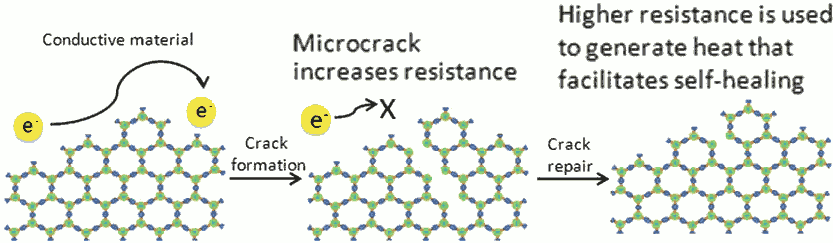
\includegraphics[width=1\textwidth]{altro/resistenza.png}}}\end{figure}
\column{0.4\linewidth}
\begin{figure}{\centering{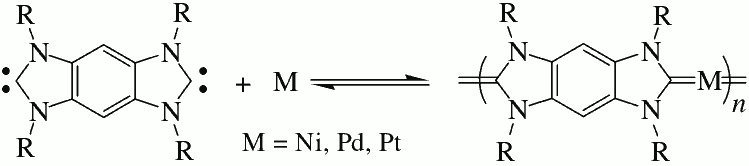
\includegraphics[width=1\textwidth]{altro/metallorganico.png}}}\end{figure}
\end{columns}
\footnote{\tiny  \fullcite{resistenza}}

\end{frame}





\subsection{Riparazione per diffusione di polimeri lineari}
\begin{frame}\frametitle{Riparazione per diffusione di polimeri lineari}

\begin{columns}
 \column{0.5\linewidth}In un polimero termoindurente viene \textbf{dissolto} in piccole quantità \textbf{un polimero termoplastico}.

\textbf{A temperatura ambiente} il polimero termoplastico \textbf{è fissato} al reticolo tramite legami ad idrogeno.

\textbf{Scaldando} e mettendo in contatto due superfici si ha sblocco e \textbf{diffusione} a riparare parzialmente la frattura.


 \column{0.5\linewidth}
\vspace{-13pt}
\begin{figure}{\centering{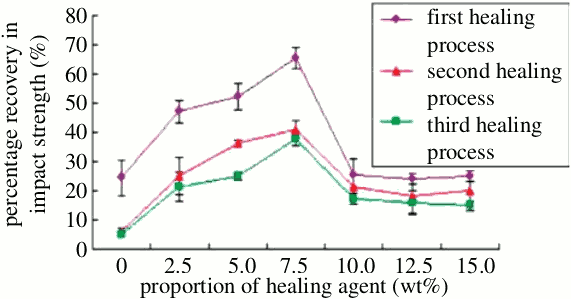
\includegraphics[width=1\textwidth]{altro/diffusione1.png}}}\end{figure}
\vspace{-20pt}
\begin{figure}{\centering{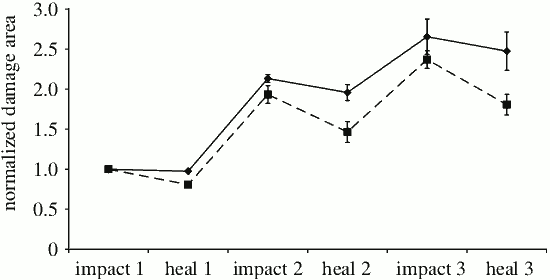
\includegraphics[width=1\textwidth]{altro/diffusione2.png}}}\end{figure}

\end{columns}
\footnote{\tiny  \fullcite{diffusione}}
\end{frame}
